% Written by Louise Fussien

% This file CAN NOT be compiled on its own
% It is included by ../Book_of_Specifications.tex


\subsection{Environnement de travail}


\subsubsection{Introduction à l'Environnement de Travail}
Dans le cadre de notre projet, nous avons choisi d'utiliser le moteur de jeu Godot en conjonction avec l'environnement de développement intégré (IDE) Rider.
Cette configuration a été sélectionnée pour ses capacités avancées en matière de développement de jeux vidéo, ainsi que pour la flexibilité et les outils de débogage puissants offerts par Rider.

\subsubsection{Fonctionnement de Godot et Intégration avec Rider}


\textbf{Godot} est un moteur de jeu open-source, reconnu pour sa facilité d'utilisation et sa capacité à gérer des projets de jeux vidéo en 2D et en 3D.
Il offre une gamme complète de fonctionnalités, y compris un éditeur visuel intuitif, des systèmes de scripting flexibles grâce à GDScript (un langage de script similaire à Python), ou C\# et des outils robustes pour l'animation et la physique.
Le choix de Godot a été motivé par sa communauté active et ses ressources abondantes, facilitant ainsi l'apprentissage et la résolution de problèmes.
\\

\textbf{Rider}, développé par JetBrains, est un IDE multiplateforme qui offre un support étendu pour de nombreux langages de programmation, notamment C\#.
Son intégration avec Godot permet d'exploiter pleinement les capacités de scripting C\# de Godot, offrant ainsi une expérience de développement plus enrichissante et productive.
Rider propose également des outils de refactoring, une navigation améliorée dans le code, et des capacités de débogage avancées, qui sont particulièrement utiles pour les projets complexes de jeux vidéo.

\subsubsection{Défis Associés aux Changements de version de Godot}

L'un des défis majeurs rencontrés dans notre environnement de travail est lié aux changements de version de Godot.
Le moteur est en constante évolution, avec des mises à jour fréquentes qui apportent de nouvelles fonctionnalités et des améliorations de performance.
Cependant, ces mises à jour peuvent également introduire des modifications significatives qui affectent la compatibilité du code existant.
\\

Pour une partie de notre groupe, moins expérimentée dans la conception de jeux vidéo, ces changements de version ont posé des problèmes d'adaptation.
Les différences entre les versions peuvent inclure des modifications dans l'API, des changements de comportement dans les outils d'animation ou de physique, et des ajustements dans les méthodes de rendu graphique.
Ces modifications nécessitent une compréhension approfondie des nouvelles fonctionnalités et des ajustements potentiellement complexes du code existant pour maintenir la stabilité et les performances du projet.
\\

Afin de surmonter ces défis, nous avons mis en place plusieurs stratégies :
\\

\begin{itemize}

      \item Documentation et Formation : Nous avons organisé des sessions de formation interne pour familiariser l'équipe avec les nouvelles fonctionnalités et les changements apportés par les mises à jour de Godot.
            Des tutoriels et des guides spécifiques ont été créés pour faciliter l'apprentissage.
            \\

      \item Environnement de Test : Avant de migrer vers une nouvelle version de Godot, nous avons établi un environnement de test dédié pour évaluer l'impact des changements sur notre projet.
            Cela nous permet de repérer et de corriger les incompatibilités potentielles avant d'intégrer les modifications dans la branche principale du projet.
            \\

      \item Révision de Code et Pair Programming : Nous avons encouragé la révision de code et le pair programming, où des membres plus expérimentés de l'équipe travaillent en étroite collaboration avec ceux moins expérimentés, pour partager des connaissances et assurer une transition en douceur entre les versions.

\end{itemize}

\subsection{Manipulation des Fichiers JSON : Défis et Solutions}

\subsubsection{Introduction à JSON et son Utilisation dans le Développement de Jeux}

JavaScript Object Notation (JSON) est un format de données léger et facile à lire et écrire pour les humains, et facile à analyser et générer pour les machines.
JSON est largement utilisé dans le développement de jeux vidéo pour stocker et échanger des données structurées. Dans notre projet, nous avons utilisé des fichiers
JSON pour stocker divers éléments du jeu, y compris des images de texte, des configurations de jeu, et des données de sauvegarde.

\subsubsection{Compréhension et Manipulation des Fichiers JSON}

Lors de notre première tentative d'intégration de fichiers JSON dans notre projet de jeu vidéo, nous avons rencontré plusieurs difficultés en raison de notre manque initial de familiarité avec ce format de fichier.
Pour remédier à cela, nous avons entrepris une étude approfondie de JSON et de ses applications dans le contexte de notre projet.

\subsubsection{Structure et Syntaxe de JSON}

JSON représente des données sous forme de paires clé/valeur et de tableaux. Une paire clé/valeur se compose d'un nom de champ (clé) et de sa valeur associée.
Les valeurs peuvent être des chaînes de caractères, des nombres, des objets (des paires clé/valeur imbriquées), des tableaux, des booléens (true/false), ou null.
\\

\begin{figure}[H]
      \centering
      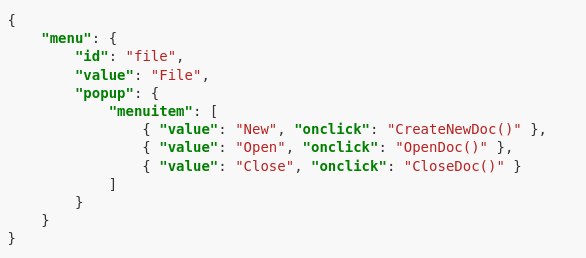
\includegraphics[width=0.8\textwidth]{assets/jsonexemple.png}
      \caption{Exemple de structure JSON}
      \label{fig:json}
\end{figure}

L'intégration de fichiers JSON dans notre code s'est révélée être un défi considérable mais stimulant.
Voici un aperçu détaillé du processus et des solutions mises en œuvre pour surmonter les obstacles techniques :
\\


\textbf{A. Lecture et Écriture de Fichiers JSON :}
\vspace*{0.2cm}

La première étape consistait à lire les données à partir des fichiers JSON et à les écrire dans ces fichiers.
Nous avons utilisé les bibliothèques de gestion des fichiers JSON disponibles dans les langages de programmation utilisés dans notre projet.
En C\#, par exemple, nous avons exploité les classes JsonSerializer et JsonDeserializer fournies par le framework .NET.
\\

\textbf{B. Sélection des Attributs à Sauvegarder :}
\vspace*{0.2cm}

Une des tâches cruciales était de déterminer quels attributs des objets de jeu devaient être sauvegardés dans les fichiers JSON.
Pour cela, nous avons effectué une analyse approfondie des besoins du jeu et de la pertinence des données à long terme.
Les attributs essentiels comme les statistiques des personnages, l'état de l'inventaire, et les positions des objets dans le monde de jeu ont été jugés importants.
En revanche, les attributs temporaires ou dérivables, comme les états intermédiaires de certaines animations, ont été exclus pour éviter un gonflement inutile des fichiers de sauvegarde.
\\

\textbf{C. Récupération des Objets à Partir de Fichiers JSON :}
\vspace*{0.2cm}

Une fois les fichiers JSON créés, la prochaine étape consistait à récupérer les objets de jeu à partir de ces fichiers.
Ce processus impliquait de désérialiser les données JSON en objets utilisables dans notre moteur de jeu.
L'un des défis majeurs ici était de garantir que les données récupérées soient correctement mappées aux structures de données de notre jeu, en respectant les types et les contraintes de chaque attribut.

\subsection{L'architecture du jeu}

L'architecture d'un projet de développement de jeux vidéo est essentielle pour assurer une organisation claire et une gestion efficace des ressources.
Dans notre projet, nous avons adopté une structure de dossiers bien définie pour faciliter la gestion des différents composants du jeu. Cette organisation
a permis de simplifier le processus de développement, de faciliter la collaboration entre les membres de l'équipe et d'assurer une maintenance efficace du code
et des ressources. Voici une description détaillée de la structure de notre projet et du rôle de chaque dossier.

\subsubsection{Structure des Dossiers}

1. Dossier Assets

Le dossier `assets` est le répertoire principal qui contient toutes les ressources visuelles et sonores utilisées dans le jeu.
Ce dossier est crucial pour centraliser toutes les images, les sons, les textures et autres médias nécessaires pour le développement du jeu.

\begin{itemize}
      \item Contenu : Images, textures, sons, et autres médias.
      \item Exemple : `assets/background.png`, `assets/music/theme.mp3`.
            \\
\end{itemize}

2. Dossier Caractères

Le dossier `caractères` est dédié aux images des personnages du jeu, incluant à la fois le joueur et les monstres.
Cette séparation permet une gestion plus facile et une localisation rapide des ressources graphiques liées aux entités interactives du jeu.

\begin{itemize}
      \item Contenu : Images des personnages joueurs et des monstres.
      \item Exemple : `caractères/joueur.png`, `caractères/monstre.png`.
            \\
\end{itemize}

3. Dossier Items

Le dossier `items` contient les fichiers JSON associés aux différents objets (items) présents dans le jeu.
Ces fichiers JSON définissent les attributs et les propriétés des objets, tels que leur nom, description, valeur, et effets en jeu.

\begin{itemize}
      \item Contenu : Fichiers JSON des objets.
      \item Exemple : `items/potion.json`, `items/épée.json`.
            \\
\end{itemize}

4. Dossier Loottables

Le dossier `loottables` est associé aux données d'objets donnés par la mort des monstres.
Ces fichiers permettent de générer les objets qui seront donnés par les monstres à leur mort.

\begin{itemize}
      \item Contenu : Fichiers JSON pour les objets des monstres.
            \\
\end{itemize}

5. Dossier Mob

Le dossier `mob` contient les fichiers JSON des monstres, décrivant leurs caractéristiques, comportements et statistiques.
Ces fichiers jouent un rôle crucial dans la définition des ennemis que les joueurs rencontreront dans le jeu.

\begin{itemize}
      \item Contenu : Fichiers JSON des monstres.
      \item Exemple : `mob/zombie.json`, `mob/dragon.json`.
            \\
\end{itemize}

6. Dossier Quest

Le dossier `quest` contient les fichiers JSON associés aux quêtes du jeu. Chaque fichier JSON représente une quête, incluant des informations telles que les objectifs, les récompenses, et les dialogues associés.

\begin{itemize}
      \item Contenu : Fichiers JSON des quêtes.
      \item Exemple : `quest/quête1.json`, `quest/quête2.json`.
            \\
\end{itemize}

7. Dossier Scenes

Le dossier `scenes` contient toutes les scènes utilisées dans le moteur Godot. Une scène dans Godot représente une collection d'objets (nodes) organisés de manière hiérarchique. Ce dossier est essentiel pour structurer les différents niveaux et interfaces du jeu.

\begin{itemize}
      \item Contenu : Fichiers de scènes Godot.
      \item Exemple : `scenes/menu.tscn`, `scenes/niveau1.tscn`.
            \\
\end{itemize}

8. Dossier Script

Le dossier `script` contient tous les scripts utilisés dans le projet. 
Ces scripts sont écrits en C\#, et sont responsables de la logique de jeu, des interactions des personnages, et des comportements des objets.

\begin{itemize}
      \item Contenu : Scripts de jeu.
\end{itemize}

\subsection{Menu du Jeu}

\begin{figure}[H]
      \centering
      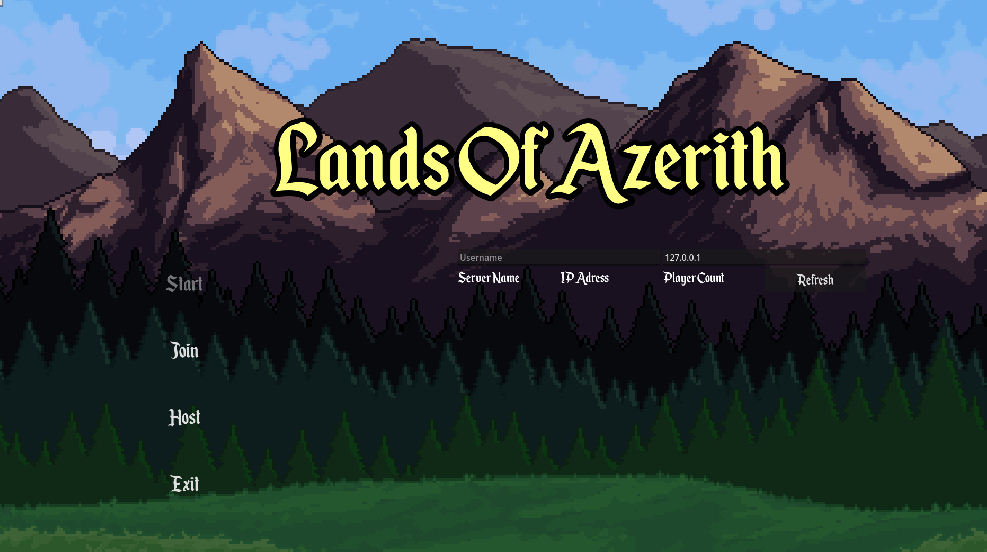
\includegraphics[width=0.8\textwidth]{assets/game_menu.png}
      \caption{Menu principal du jeu}
      \label{fig:game_menu}
\end{figure}

\subsubsection{Introduction à l'Effet Parallax dans le Menu}

L'effet parallax est une technique visuelle utilisée pour créer une sensation de profondeur en animant différents plans à des vitesses différentes.
Dans notre jeu, nous avons implémenté un effet parallax dans le menu principal pour donner une impression de perspective en 2D.
Voici comment nous avons structuré et mis en œuvre cet effet de manière efficace et immersive.

\subsubsection{Implémentation de l'Effet Parallax}

Nous avons créé une node principale ParallaxBackground dans Godot, qui agit comme le conteneur global pour notre effet parallax.
Cette node a des enfants (fils) correspondant à chaque plan de fond que nous voulons animer. Chaque plan a une image différente et une vitesse de défilement spécifique, ce qui crée une illusion de profondeur lorsque le joueur navigue dans le menu.

\subsubsection{Structure de la Node ParallaxBackground}

La node ParallaxBackground est configurée avec plusieurs enfants (fils), chacun représentant un plan de fond distinct.
Chaque plan est un sprite ou une texture avec une image unique et est déplacé à une vitesse différente par rapport aux autres plans pour simuler la perspective.
\\

\begin{figure}[H]
      \centering
      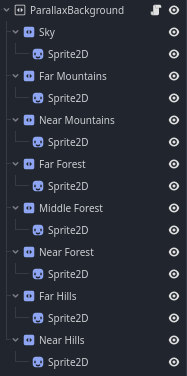
\includegraphics[width=0.3\textwidth]{assets/paralax.png}
      \caption{Exemple de structure de la node ParallaxBackground}
      \label{fig:paralax}
\end{figure}

\subsubsection{Animation et Effet Visuel}

Chaque plan de fond est animé en ajustant sa position horizontale à chaque trame (frame) du jeu, en fonction de sa vitesse définie.
Les plans plus proches (vitesse plus faible) se déplacent plus lentement par rapport à ceux qui sont plus éloignés (vitesse plus élevée),
créant ainsi un effet de parallaxe réaliste qui renforce l'immersion du joueur dès le lancement du jeu.

\subsection{Le Multijoueur}

Pour pouvoir organiser une partie multijoueur, nous avons décidé d'utiliser l'API intégrée à Godot.
Pour cela, il nous faut un serveur, ici l'hôte, ainsi que les joueurs qui rejoignent sa partie appelés les clients,
En premier temps, l'hôte doit appuyer sur le bouton 'Host' puis les joueurs doivent accéder à l'adresse de l'hôte, et appuyer sur le bouton 'Join'.
\\

Il est possible de jouer avec un nombre infini de joueurs, mais nous avons établi un maximum de 8, limite que nous utiliserons lors de la conception du reste du jeu.
\\

Maintenant que la connexion est établie entre les différents joueurs, il nous faut synchroniser leurs informations entre eux,
tout en faisant attention à ne pas trop partager d'informations inutiles, pour limiter l'utilisation de bande passante.
Par exemple, la synchronisation des positions de chacun entre tous les joueurs est importante,
mais la position de la caméra d'un joueur n'est nécessaire qu'en local.

\subsubsection{Système de Connexion Multi-joueurs via Envoi de Paquets}

Pour permettre une connectivité multi-joueurs fluide et intuitive, nous avons implémenté un système de gestion de serveur et de connexion basé sur l'envoi de paquets.
Ce système est conçu pour simplifier l'expérience des joueurs en éliminant la nécessité d'entrer manuellement les adresses IP des serveurs.

\subsubsection{Fonctionnement du Système}

\textbf{A. Serveur d'Hébergement :}
\vspace*{0.2cm}

Lorsqu'un joueur décide d'héberger une partie, le jeu démarre un serveur local et commence à envoyer des paquets d'informations à intervalles réguliers
(par exemple, toutes les secondes).
Chaque paquet contient des détails essentiels comme le nom du serveur, l'adresse IP du serveur, et le nombre actuel de joueurs connectés.
\\

\textbf{B. Joueurs Rejoignant le Serveur :}
\vspace*{0.2cm}

Les autres joueurs du réseau écoutent en permanence les paquets émis par les serveurs disponibles.
Lorsqu'un paquet est détecté, les détails du serveur sont affichés à l'écran, permettant aux joueurs de visualiser facilement les serveurs disponibles ainsi que les informations pertinentes comme le nom et le nombre de joueurs.
Un bouton "Rejoindre" est proposé aux joueurs pour se connecter au serveur sélectionné, simplifiant ainsi le processus de connexion.
\\

\textbf{C. Démarrage de la Partie :}
\vspace*{0.2cm}

Une fois que les joueurs se sont connectés au serveur et que le nombre requis est atteint, un bouton "Start" devient accessible à tous les participants.
Lorsque tous les joueurs ont cliqué sur "Start", la partie commence, permettant ainsi de synchroniser l'expérience de jeu pour tous les participants.

\subsubsection{Avantages du Système de Paquets}

Ce système de connexion basé sur l'envoi de paquets présente plusieurs avantages :
\\

\begin{itemize}
      \item Simplicité d'utilisation : Les joueurs n'ont pas besoin de connaître l'adresse IP du serveur manuellement.
            \\

      \item Visibilité et Accessibilité : Les informations sur les serveurs disponibles sont clairement affichées, facilitant ainsi la sélection et la connexion.
            \\

      \item Synchronisation Facile : Tous les joueurs sont automatiquement informés des détails du jeu en cours, assurant ainsi une expérience de jeu fluide et harmonieuse.
\end{itemize}

\subsection{Contrôles et Interaction dans le Jeu}

Les contrôles et interactions jouent un rôle crucial dans l'expérience de jeu, assurant une navigation fluide et intuitive à travers l'environnement virtuel.
Dans notre jeu développé sous Godot, nous avons mis en œuvre plusieurs fonctionnalités de contrôle permettant aux joueurs de se déplacer d'interagir avec l'environnement, de gérer leur inventaire et de lancer des actions spécifiques avec facilité.
\\

Les déplacements du joueur sont gérés à l'aide des touches Z, Q, S, et D, qui correspondent respectivement aux directions Haut, Gauche, Bas, et Droite sur le clavier.
Cette configuration permet une navigation fluide dans les différents niveaux du jeu.
L'utilisation de la librairie d'entrée de Godot facilite la détection des touches pressées et assure une réponse instantanée aux actions du joueur.

\subsubsection{Actions Spécifiques}

\textbf{A. Quitter le Jeu avec la Touche Échap}
\vspace*{0.2cm}

Pour offrir une sortie rapide et intuitive du jeu, la touche Echap est associée à la fonction de fermeture de l'application.
Cela permet aux joueurs de quitter le jeu à tout moment sans effort, tout en libérant proprement toutes les ressources utilisées par le jeu.
\\

\textbf{B. Courir avec la Touche Shift}
\vspace*{0.2cm}

La touche Majuscule est utilisée pour activer le mode de course du joueur, augmentant ainsi sa vitesse de déplacement.
Ce mécanisme permet aux joueurs de se déplacer plus rapidement lorsqu'ils ont besoin d'atteindre des destinations plus éloignées ou de fuir des dangers potentiels dans le jeu.
\\

\textbf{C. Ouvrir l'Inventaire avec la Touche Tab}
\vspace*{0.2cm}

L'inventaire est une composante essentielle de nombreux jeux, offrant aux joueurs la possibilité de gérer leurs objets, équipements et ressources.
Dans notre jeu, l'inventaire est accessible en appuyant sur la touche Tab, facilitant ainsi la gestion des items collectés et des équipements utilisés par le joueur.
\\

\textbf{D. Attaquer avec le Clic Gauche de la Souris}
\vspace*{0.2cm}

Pour interagir avec les monstres et autres éléments interactifs dans le jeu, les joueurs peuvent utiliser le clic gauche de la souris.
Ce mécanisme permet de lancer des attaques, d'activer des objets ou d'interagir avec des éléments du décor, offrant ainsi une expérience immersive et dynamique.
\\

\textbf{E. Implémentation Technique}
\vspace*{0.2cm}

Chaque fonctionnalité de contrôle est implémentée en utilisant les capacités intégrées de Godot pour gérer les événements d'entrée et les interactions utilisateur.
Cette approche assure une cohérence dans le traitement des actions du joueur et garantit une jouabilité fluide et intuitive tout au long du jeu.

\subsection{Intelligence Artificielle : Comportements des Monstres}

Dans notre jeu, nous avons implémenté différents comportements pour les monstres afin d'enrichir l'interaction avec le joueur.
Chaque type de monstre possède des caractéristiques et des réactions spécifiques, déterminées par une classe dédiée qui gère son comportement en fonction des interactions avec le joueur.

\subsubsection{Types de Monstres}

Nous avons défini quatre types de monstres, chacun ayant un comportement distinct en fonction de la proximité et des actions du joueur :
\\

\begin{itemize}
      \item Agressif :
            Ce type de monstre attaque activement le joueur dès qu'il est à proximité.
            Lorsque le joueur entre dans sa zone de détection, le monstre commence à se déplacer vers le joueur pour l'attaquer.
            En cas de contact avec le joueur, le monstre déclenche une attaque ou une réaction offensive.
            \\

      \item Neutre :
            Les monstres neutres ne sont pas agressifs par nature mais répondent si le joueur les attaque.
            Lorsque le joueur les agresse, ils changent leur comportement pour devenir agressifs et attaquent en retour.
            En dehors des attaques contre eux, ils continuent leurs activités normales sans réaction offensive.
            \\

      \item Passif :
            Les monstres passifs ne cherchent pas à attaquer le joueur et fuient s'il est agressé.
            Lorsque le joueur les attaque, ils s'éloignent activement du joueur pour éviter tout contact et toute confrontation directe.
            \\

      \item Peureux :
            Les monstres peureux évitent activement tout contact avec le joueur.
            Dès que le joueur s'approche, ils tentent de s'éloigner rapidement et de fuir la zone de danger.

\end{itemize}

\subsubsection{Implémentation Technique}

Chaque type de monstre est implémenté à l'aide de classes distinctes dans Godot, chacune étant responsable de la gestion des comportements spécifiques décrits ci-dessus.
Voici comment nous avons mis en œuvre ces comportements complexes à l'aide des capacités de détection de collisions et de signaux de Godot :
\\

\textbf{A. Détection de Collision avec CollisionShape2D}
\vspace*{0.2cm}

Chaque monstre est équipé d'une CollisionShape2D dans Godot, configurée pour détecter les collisions avec le joueur et d'autres entités du jeu.
Cette forme de collision est essentielle pour déclencher des actions basées sur la proximité et les interactions spatiales avec d'autres nodes dans la scène.
\\

\textbf{B. Utilisation de Area2D pour les Signaux}
\vspace*{0.2cm}

Nous utilisons également des nodes Area2D pour émettre des signaux vers la node principale du monstre.
Ces signaux sont utilisés pour détecter quand le joueur entre dans la zone de détection du monstre, ce qui déclenche un changement de comportement en fonction du type de monstre :
\\

Pour les monstres agressifs et neutres : lorsque le joueur entre dans la zone, le monstre commence à se déplacer vers le joueur pour l'attaquer (si neutre, il attaque en retour si attaqué).
Pour les monstres passifs et peureux : lorsque le joueur entre dans la zone, le monstre s'éloigne activement du joueur pour éviter le contact.
\\

\textbf{C. Gestion des Comportements Dynamiques}
\vspace*{0.2cm}

Chaque classe de monstre gère de manière dynamique son comportement en réponse aux signaux émis par Area2D.

\begin{figure}[H]
      \centering
      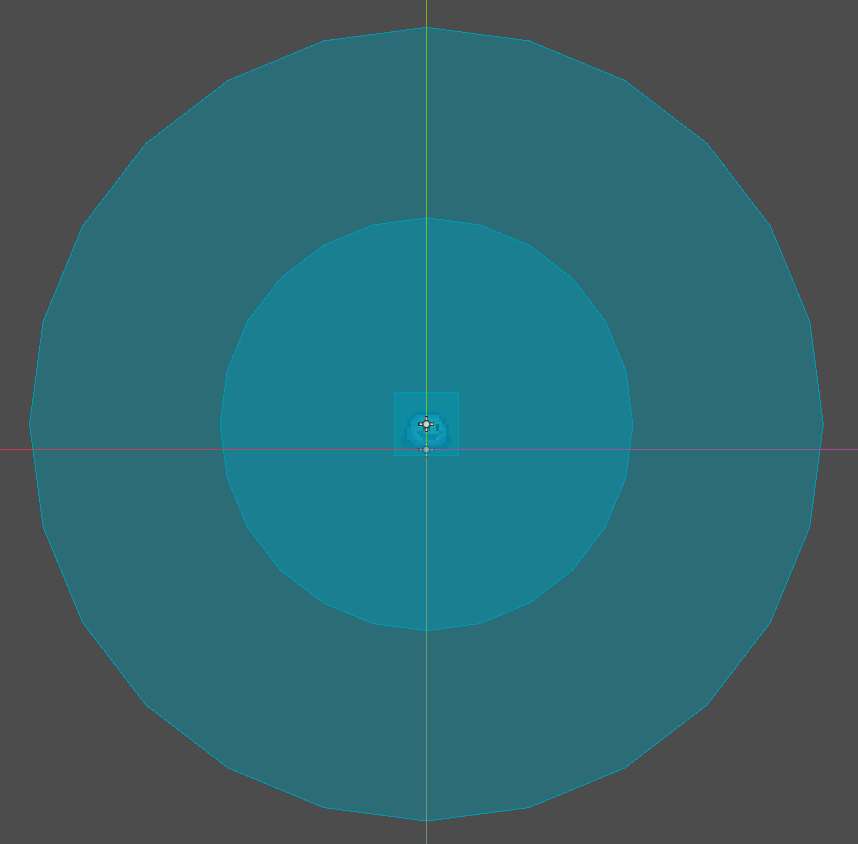
\includegraphics[width=0.6\textwidth]{assets/mob.png}
      \caption{Exemple du signal émis par le mob}
      \label{fig:website1}
\end{figure}

\subsection{Déplacement des Monstres avec Navigation A*}

Dans notre jeu, nous avons intégré des mécanismes avancés pour le déplacement des monstres en utilisant le système de navigation A* (A-star) et
la gestion de l'inventaire du joueur.
Ces fonctionnalités améliorent l'expérience de jeu en offrant des déplacements fluides et des interactions riches avec les objets collectés. Voici comment nous avons implémenté ces fonctionnalités techniques dans Godot.

\subsubsection{Algorithme A*}

Pour permettre aux monstres de se déplacer intelligemment dans l'environnement du jeu, nous avons utilisé la node \texttt{Navigation2D} de Godot, qui intègre un système de pathfinding basé sur l'algorithme A*.
Cela permet aux monstres de calculer automatiquement le chemin le plus optimal vers leur cible, comme le joueur ou un point spécifique de la carte.

\subsubsection{Implémentation de la Node \texttt{Navigation2D}}

La node \texttt{Navigation2D} est configurée pour représenter la carte jouable du jeu, avec des obstacles et des zones de passage définies. Voici comment elle est utilisée dans Godot :
\\

\begin{itemize}
      \item \textbf{Configuration de la Navigation} :
            Nous avons généré une carte de navigation en plaçant des obstacles et en définissant les zones accessibles par les monstres.
            Cette carte est utilisée par l'algorithme A* pour calculer les chemins.
            \\

      \item \textbf{Utilisation de \texttt{Navigation2D} dans le Code} : Chaque monstre
            est doté d'une instance de \texttt{Navigation2D}, configurée pour calculer un chemin vers sa cible actuelle à intervalles réguliers.
\end{itemize}

\subsubsection{Déplacement Dynamique des Monstres}

À intervalles réguliers, les monstres recalculent leur chemin vers leur cible (par exemple, le joueur) en utilisant la fonctionnalité
de \texttt{Navigation2D}. Cela garantit que les monstres peuvent naviguer efficacement autour des obstacles et trouver le chemin le plus court pour atteindre leur objectif.

\subsubsection{Aléatoire dans le Rayon de Déplacement}

Pour ajouter une variabilité aux déplacements des monstres, toutes les 5 secondes, chaque monstre a une chance sur trois de choisir une nouvelle destination aléatoire à l'intérieur d'un rayon de 300 pixels autour de sa position actuelle. 
Cela simule un comportement plus organique et imprévisible des monstres, rendant leur présence dans le jeu plus dynamique et réaliste.

\subsubsection{Spawning des Monstres dans une Zone Définie}

Pour enrichir l'exploration du joueur et maintenir la dynamique du jeu, nous avons mis en place un système de spawn de monstres dans des zones prédéfinies :
\\

\begin{itemize}
      \item \textbf{Zone de Spawn Rectangulaire} : Nous avons défini une zone rectangulaire dans la carte du jeu où les monstres peuvent apparaître périodiquement.
            \\

      \item \textbf{Instantiation des Monstres} : Toutes les 15 secondes, un nouveau monstre est instancié dans cette zone de spawn si la limite de monstres dans
            cette zone n'est pas atteinte.
            \\

      \item \textbf{Chargement Dynamique depuis un Fichier JSON} : Chaque type de monstre est associé à un fichier
            JSON qui contient ses caractéristiques, comme ses attributs, ses comportements et ses statistiques. Lorsqu'un monstre est instancié,
            ces informations sont chargées à partir du fichier JSON correspondant.
\end{itemize}

\subsection{Gestion de l'inventaire du joueur }

\subsubsection{Structure de l'Inventaire}

L'inventaire est représenté par un tableau de cases, où chaque case peut contenir un objet spécifique avec sa quantité.
Les joueurs peuvent visualiser leur inventaire en appuyant sur la touche \texttt{Tab}, ce qui ouvre une interface utilisateur affichant
les objets collectés et leur quantité respective.

\subsubsection{Interaction avec l'Inventaire}

\begin{itemize}
      \item \textbf{Ajout d'Objets} : Lorsque le joueur ramasse un nouvel objet, celui-ci est ajouté à l'inventaire s'il n'est pas déjà présent.
            Si l'objet est déjà présent, la quantité existante est simplement mise à jour.
            \\
      \item \textbf{Affichage et Gestion} : L'interface de l'inventaire permet aux joueurs de visualiser, utiliser et organiser leurs objets selon
            leurs besoins. Par exemple, les objets peuvent être équipés, consommés ou échangés selon leur utilité dans le jeu.
\end{itemize}

\subsection{Gestion des Points de Vie, Checkpoints et Loot dans le Jeu}

Dans notre jeu, nous avons mis en place un système robuste pour gérer les points de vie du joueur, les checkpoints pour la réapparition, et la mécanique de loot des monstres. Voici comment chaque aspect est implémenté pour enrichir l'expérience de jeu et assurer une progression gratifiante pour les joueurs.

\subsubsection{Points de Vie du Joueur}

Le joueur démarre avec un nombre initial de points de vie (PV) fixé à 1000. Lorsqu'il subit une attaque de la part d'un monstre ou d'un autre ennemi, les dégâts infligés sont calculés en fonction de la force de l'attaque et des attributs de l'arme de l'attaquant.

\subsubsection{Calcul des Dégâts}

Les dégâts subis par le joueur sont calculés en fonction de la formule suivante, basée sur la force de l'attaque (\textit{force\_attaque}) et le nombre de points de l'arme (\textit{points\_arme}) de l'attaquant : (\textit{points\_arme}) + (\textit{force\_attaque})
\\

Cela permet d'ajuster dynamiquement les dégâts en fonction de la puissance de l'attaque et de l'équipement de l'attaquant, ajoutant ainsi une couche de stratégie et de gestion des ressources pour le joueur.

\subsubsection{Gestion des Checkpoints}

Pour assurer une progression fluide et éviter une perte de progrès significative en cas de mort du joueur, nous avons intégré un système de checkpoints :
\\

\begin{itemize}
      \item \textbf{Réapparition au Dernier Checkpoint} : Lorsque le joueur meurt, il réapparaît au dernier checkpoint atteint. Cette fonctionnalité est essentielle pour réduire la frustration du joueur et encourager l'exploration sans crainte de perdre tout son progrès.
            \\

      \item \textbf{Restauration des Points de Vie Maximum} : À chaque réapparition, le joueur récupère ses points de vie maximum, lui permettant de reprendre le jeu avec une chance égale de succès.
\end{itemize}

\subsubsection{Mécanique de Loot des Monstres}

Lorsqu'un monstre est vaincu, plusieurs actions se produisent pour enrichir l'expérience du joueur :
\\
\begin{itemize}
      \item \textbf{Loot des Objets Associés au Monstre} : Chaque type de monstre est associé à un fichier JSON définissant les objets qu'il peut lâcher lorsqu'il meurt. Ces objets peuvent inclure des équipements, des ressources ou d'autres items précieux pour la progression du joueur.
            \\

      \item \textbf{Apparition de Débris et Textures} : Pour indiquer visuellement la mort du monstre, des débris et des textures spécifiques à ce monstre apparaissent à l'emplacement où il a été vaincu. Cela crée une immersion et une satisfaction visuelle pour le joueur.
            \\

      \item \textbf{Récupération des Objets par le Joueur} : Lorsque le joueur passe sur les débris et textures laissés par le monstre, il récupère automatiquement les objets associés dans son inventaire. Cela simplifie le processus de collecte et de gestion des objets obtenus lors des combats.
\end{itemize}

\subsection{Génération de Map et Gestion des Transitions avec Nodes dans Godot}

Dans notre jeu, la création et la gestion des textures de la carte ainsi que les transitions fluides entre les différents environnements sont
des aspects cruciaux pour offrir une expérience visuelle immersive et dynamique.
Voici comment nous avons implémenté ces fonctionnalités techniques avancées dans Godot, en nous concentrant sur la génération de la carte, les transitions entre les maps et l'animation des personnages et des objets.

\subsection{Génération de la Map et Utilisation des Textures}

La carte du jeu est entièrement générée et dessinée par notre designer, ce qui nous permet de contrôler précisément l'aspect visuel et le design de chaque environnement.
Voici comment nous avons structuré notre approche :

\subsubsection{Textures et Tiles}

Pour la création de la carte, nous utilisons des textures organisées en tiles.
Chaque tile représente une partie spécifique de la carte, telle que le sol et les éléments statiques qui ne bougent pas.
Ces textures sont soigneusement intégrées dans la map pour former des environnements cohérents et esthétiquement plaisants.

\subsubsection{Tileset pour les Maps}

Les tilesets sont des images contenant plusieurs textures utilisées pour les maps. Ils permettent de définir les décors,
les détails du sol et d'autres éléments fixes qui ne changent pas pendant le jeu. Cela garantit une cohérence visuelle et simplifie
la gestion des textures dans l'environnement du jeu.

\begin{figure}[H]
      \centering
      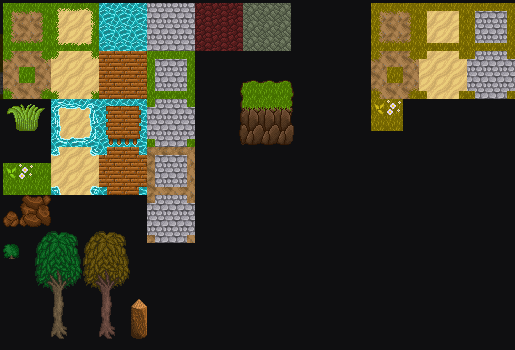
\includegraphics[width=0.8\textwidth]{assets/tileset.png}
      \caption{Nos textures}
      \label{fig:website1}
\end{figure}

\subsection{Gestion des Transitions entre les Maps}

Les transitions entre les différentes zones de la carte sont gérées à l'aide de nodes spécifiques qui assurent une expérience de jeu fluide et immersive :

\subsubsection{Nodes de Transition}

Chaque zone de transition est représentée par une node comportant un \texttt{Area2D} et une \texttt{CollisionShape2D}.
Lorsque le joueur entre dans cette zone, des événements sont déclenchés pour faire apparaître la nouvelle map, faire disparaître l'ancienne et ajuster les coordonnées du joueur, créant ainsi une illusion de téléportation fluide et réaliste.

\subsubsection{Changement Dynamique de la Map}

Lorsque le joueur traverse une zone de transition, le jeu procède à un chargement dynamique de la nouvelle map tout en déchargeant celle précédente. 
Cela permet de maintenir une utilisation efficace des ressources tout en offrant une navigation sans heurts à travers les différentes zones de jeu.

\subsection{Animation des Personnages et des Objets}

Pour donner vie aux personnages et aux objets dans notre jeu, nous utilisons des animations basées sur des sprites animés (\texttt{AnimatedSprite2D}). 
Ces animations sont essentielles pour créer des mouvements fluides et réalistes :

\subsubsection{Sprites Animés}

Chaque personnage, monstre et objet interactif est doté d'un \texttt{AnimatedSprite2D} qui contient une séquence d'images.
Ces images sont affichées successivement selon un rythme prédéfini, créant ainsi des animations telles que la marche, la course, l'attaque ou d'autres actions spécifiques.

\subsubsection{Création de Mouvements}

Les animations des personnages sont conçues pour refléter leur comportement et leurs actions dans le jeu. 
Par exemple, un personnage pourrait avoir une animation pour lever son arme avant de frapper, ou une animation de marche où les images des pieds gauche et droit sont alternées pour simuler le mouvement.
\\

En intégrant ces techniques avancées de gestion de textures, de transitions de maps et d'animation dans notre jeu sous Godot, nous avons réussi à créer une expérience de jeu immersive et visuellement attrayante. 
La génération de maps et l'utilisation de tilesets garantissent une conception précise et esthétique des environnements, tandis que les transitions fluides et les animations dynamiques des personnages enrichissent l'expérience globale du joueur. 
Cette approche technique non seulement améliore la jouabilité mais aussi renforce l'engagement des joueurs envers notre univers de jeu, offrant ainsi une expérience mémorable et captivante à chaque session de jeu.

